\documentclass[xcolor=dvipsnames]{beamer}
\usetheme{Madrid}


\setbeamertemplate{navigation symbols}{}
%\setbeamertemplate{headline}{}

%\setbeamertemplate{frametitle}{\insertpagenumber}
\setbeamertemplate{footline}[frame number]
%\setbeamersize{text margin left=7mm}
%\setbeamersize{text margin right=7mm}

\usepackage{hyperref}
%\hypersetup{colorlinks, linkcolor=black}

\usepackage{times}

\usepackage{xltxtra}
\setsansfont{Calibri}
\setmonofont{Consolas}

\usepackage{minted}


\author{Jan Dědek}

\institute[MFF UK] % (optional, but mostly needed)
{
  Department of Software Engineering\\
	Faculty of Mathematics and Physics\\
	Charles University in Prague
}

\date[DEDEK-PHD, 2012]
{
Defence of Doctoral Thesis\\21\textsuperscript{st} September\\2012
}

\title{Semantic Annotations}

\begin{document}

\begin{frame}
  \titlepage
\end{frame}

\definecolor{DarkGreen}{rgb}{0,.392,0}
\definecolor{DarkMagenta}{rgb}{.545,0,.545}
\definecolor{DarkCyan}{rgb}{0,.545,.545}


\def \colorManual    {Brown}
\def \colorLearning  {DarkGreen}
\def \colorShareable {DarkCyan}
\def \colorFuzzy     {DarkMagenta}
\def \mysetbeamercolor [#1]#2 {\setbeamercolor{#1}{fg=#2}}

\mysetbeamercolor[colorManual]{\colorManual}
\mysetbeamercolor[colorLearning]{\colorLearning}
\mysetbeamercolor[colorShareable]{\colorShareable}
\mysetbeamercolor[colorFuzzy]{\colorFuzzy}


\def \themecolor #1 {\setbeamercolor*{titlelike}{parent=palette primary, bg=#1}}
\def \themetext [#1]#2 {{\usebeamercolor{#1}{\color{fg}\textbf{#2}}}}
\def \resetcolor {\setbeamercolor*{titlelike}{parent=palette primary}}



\definecolor{mybkg}{RGB}{240,240,240}
\setbeamercolor{block title}{bg=OliveGreen}
\setbeamercolor{block body}{bg=mybkg}

\begin{frame}{Outline}
  \tableofcontents
\end{frame}

\section{Introduction} 
\subsection{Information Extraction} 
\frame{\tableofcontents[currentsubsection]}
\begin{frame}{Information Extraction (Problem)}  
\begin{itemize}
	\item Let's have a text describing an acquisition event.
	\medskip
	\framebox{\includegraphics[width=0.6\hsize]{img/acquisitions_plain.png}}
	\item What was the object of the acquisition?
	\item Who was the buyer?
	\item What was the deal amount?
\end{itemize}
\end{frame}

\begin{frame}{Information Extraction (Solution)}  
\begin{itemize}
	\item Information Extraction tools can identify and extract such information.
	%\begin{itemize}
		%\item Of course not 100\% accurete...
	%\end{itemize}
	\medskip
	\framebox{\includegraphics[width=0.85\hsize]{img/acquisitions_annotated.png}}
	%\item The tools can also interpret such information in terms of a \alert{Semantic Web Ontology}.
\end{itemize}
\end{frame}

\begin{frame}{Information Extraction (Czech Example)}  
\begin{itemize}
	\item Information Extraction tools can identify and extract such information.
	%\begin{itemize}
		%\item Of course not 100\% accurete...
	%\end{itemize}
	\medskip
	\includegraphics[width=0.85\hsize]{img/fireman_annotated}
	%\item The tools can also interpret such information in terms of a \alert{Semantic Web Ontology}.
\end{itemize}
\end{frame}

\subsection{Deep Language Parsing} 
\begin{frame}{Deep Language Parsing (Czech Example)}  
\begin{itemize}
	\item Linguistic tools perform automated linguistic analysis.
	\item Producing so called \emph{dependency trees}.
	%\begin{itemize}
		%\item Of course not 100\% accurete...
	%\end{itemize}
	\medskip
	\framebox{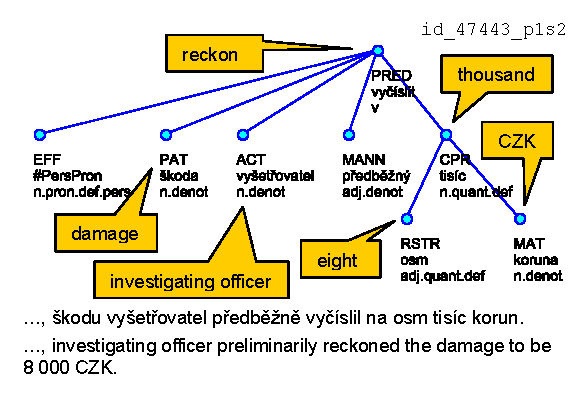
\includegraphics[width=0.85\hsize]{img/tree}}
	%\item The tools can also interpret such information in terms of a \alert{Semantic Web Ontology}.
\end{itemize}
\end{frame}

\subsection{Inductive Logic Programming} 

\begin{frame}{Inductive Logic Programming}
\begin{itemize}
	\item Learning examples $E=P\cup N$ (Positive and Negative)	
	\begin{itemize}
		\item E.g. relevant and irrelevant pieces of text w.r.t. particular extraction task
	\end{itemize}	
	\item Background knowledge $B$
	\begin{itemize}
		\item E.g. linguistic structure connecting individual words
	\end{itemize}	
	\item ILP task: To find logical program or hypothesis $H$ such that all positive examples are covered and none negative
$$
(\forall e\in P)(B\cup H\models e) \ \ \&\  \ (\forall n\in N)(B\cup H\not\models n).
$$
	\begin{itemize}
		\item E.g. to find common pattern (in the linguistic structure) present around every relevant piece of text and none irrelevant.
	\end{itemize}	
\end{itemize}
\end{frame}


\subsection{Organization of this Presentation} 
\frame{\tableofcontents[currentsubsection]}

\begin{frame}{Four Main Topics}

\begin{itemize}
	\item \themetext[colorManual]{Manual Design of Extraction Rules}
	\item \themetext[colorLearning]{Induction of Extraction Rules}
	\item \themetext[colorShareable]{Shareable Extraction Ontologies}
	\item \themetext[colorFuzzy]{Fuzzy ILP Document Classification}
\end{itemize}

\end{frame}


\themecolor{\colorManual}
\begin{frame}{Manual Design of Extraction Rules}
Slides about the topic \emph{Manual Design of Extraction Rules} will have \themetext[colorManual]{brown }  headline background.
\end{frame}

\themecolor{\colorLearning}
\begin{frame}{Induction of Extraction Rules}
Slides about the topic \emph{Induction of Extraction Rules} will have \themetext[colorLearning]{green }  headline background.
\end{frame}

\themecolor{\colorShareable}
\begin{frame}{Shareable Extraction Ontologies}
Slides about the topic \emph{Shareable Extraction Ontologies} will have \themetext[colorShareable]{cyan }  headline background.
\end{frame}

\themecolor{\colorFuzzy}
\begin{frame}{Fuzzy ILP Document Classification}
Slides about the topic \emph{Fuzzy ILP Document Classification} will have \themetext[colorFuzzy]{magenta }  headline background.
\end{frame}

\resetcolor
\begin{frame}{Ordinary}
\end{frame}


\section{Contents}
\frame{\tableofcontents[currentsection]}

\section[Questions \& Comments]{Questions and Comments from Reviews} 
\frame{\tableofcontents[currentsection]}

\end{document}
